\documentclass{eeleyes}

\usepackage{fancyhdr}
\pagestyle{fancy}
\fancyhead[lcr]{}
\fancyhead[l]{Eli Griffiths}
\fancyhead[c]{MATH $140$C}
\fancyhead[r]{HW \#$2$}

\usepackage{multicol}

\newcommand\conj[1]{\overline{#1}}
\newcommand\term[1]{\textbf{#1}}
\newcommand\eps{\varepsilon}
\DeclareMathOperator{\interior}{int}

\begin{document}

\section*{Problem 1}
\begin{enumerate}[label=\alph*)]
    \item
        Consider some $(x, y) \in S$. Suppose towards contradiction there is a nbhd $V$ of $(x,y)$ such that $V \subseteq S$. Since $V$ is open, there must be an open ball of some radius $r$ such that $B_r((x,y)) \subseteq V$. Between $x$ and $x+r$ must be some irrational $i$, and since $x - i < r$, $(i, y) \in S$. However $i \notin \Q$, a contradiction. Therefore $\interior(\Q) = \varnothing$.
    \item 
        The boundary of a set is simply its closure minus its interior. The closure of the rationals is the reals, and since $\interior(\Q) = \varnothing$, $\partial \Q = \R \setminus \varnothing = \R$.
\end{enumerate}

\section*{Problem 2}
Yes.
\begin{proof}
    Let $S \subseteq \R^n$ be bounded. That is $\exists M > 0$ such that $\norm{x} \leq M$ for all $x \in S$. Pick $x \in \conj{S}$. If $x \in S$, then since $S$ is already bounded $\norm{x} \leq M$. Therefore consider when $x \in \conj{S}$ but $x \notin \conj{S}$. Then $x$ is a cluster point of $S$ meaning there exists some sequence $\qty(x^{(k)})$ in $S$ such that $\lim x^{(k)} = x$. Therefore there is some $K$ such that for any $k \geq K$, $\norm{x_k - x} \leq 1$. Note then that for $k \geq K$
    \[
        \norm{x} = \norm{x - x_k + x_k} \leq \norm{x_k} + \norm{x_k - x} \leq M + 1
    \]
    since $x_k \in S$ and hence $\norm{x} \leq M + 1$. Thus taking the bound $\tilde{M} = M + 1$ bounds all points in $\conj{S}$.
\end{proof}

\section*{Problem 3}
\subsection*{i}
\begin{multicols}{3}
\begin{center}
    \[
        \interior(E)
    .\]
    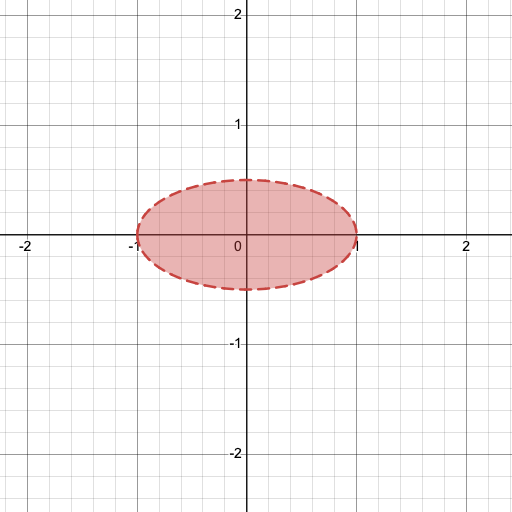
\includegraphics[width=0.8\linewidth]{figures/i_img-1.png}
\end{center}

\columnbreak

\begin{center}
    \[
        \conj{E}
    .\]
    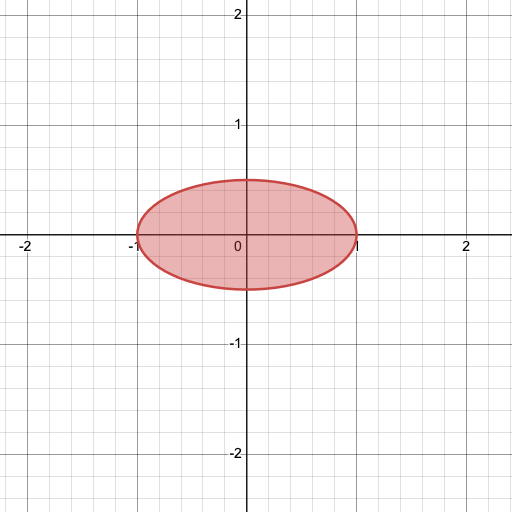
\includegraphics[width=0.8\linewidth]{figures/i_img-2.png}
\end{center}

\columnbreak

\begin{center}
    \[
        \partial E
    .\]
    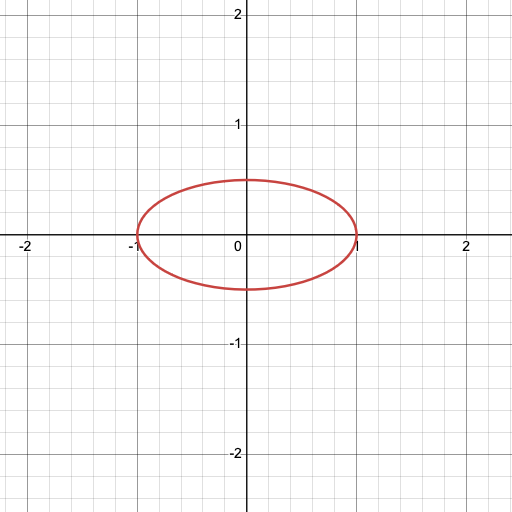
\includegraphics[width=0.8\linewidth]{figures/i_img-3.png}
\end{center}
\end{multicols}

\subsection*{ii}
\begin{multicols}{3}
\begin{center}
    \[
        \interior(E)
    .\]
    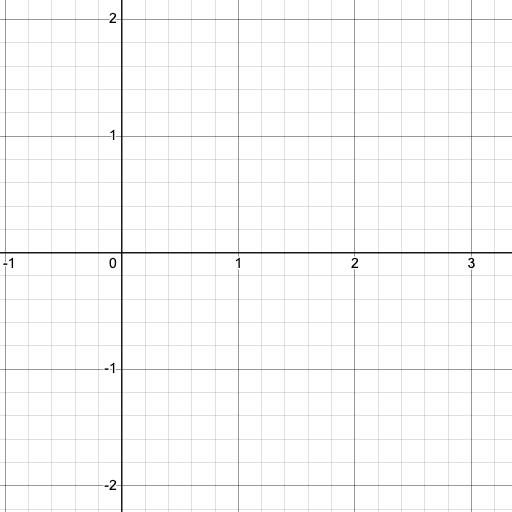
\includegraphics[width=0.8\linewidth]{figures/ii_img-1.png}
\end{center}

\columnbreak

\begin{center}
    \[
        \conj{E}
    .\]
    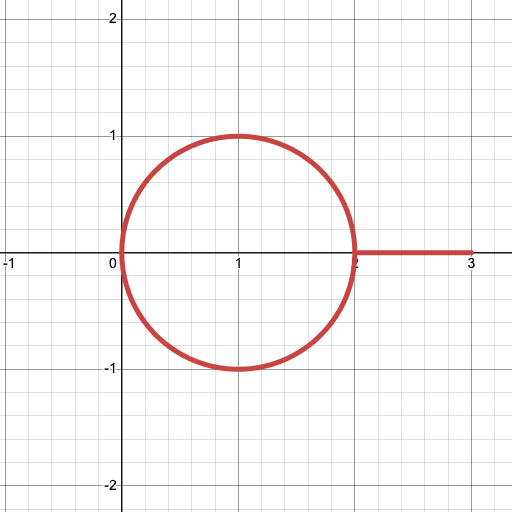
\includegraphics[width=0.8\linewidth]{figures/ii_img-3.png}
\end{center}

\columnbreak

\begin{center}
    \[
        \partial E
    .\]
    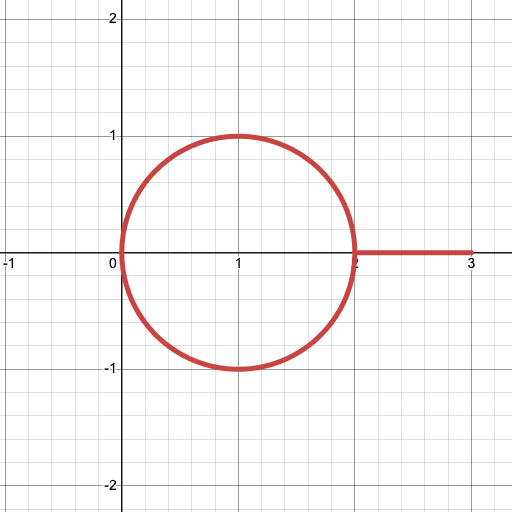
\includegraphics[width=0.8\linewidth]{figures/ii_img-3.png}
\end{center}
\end{multicols}

\subsection*{iii}
\begin{multicols}{3}
\begin{center}
    \[
        \interior(E)
    .\]
    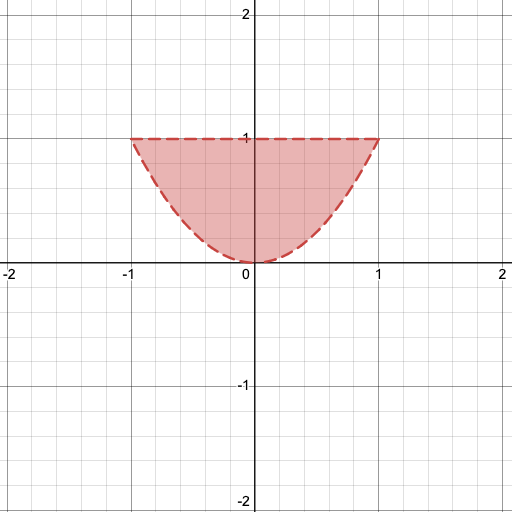
\includegraphics[width=0.8\linewidth]{figures/iii_img-1.png}
\end{center}

\columnbreak

\begin{center}
    \[
        \conj{E}
    .\]
    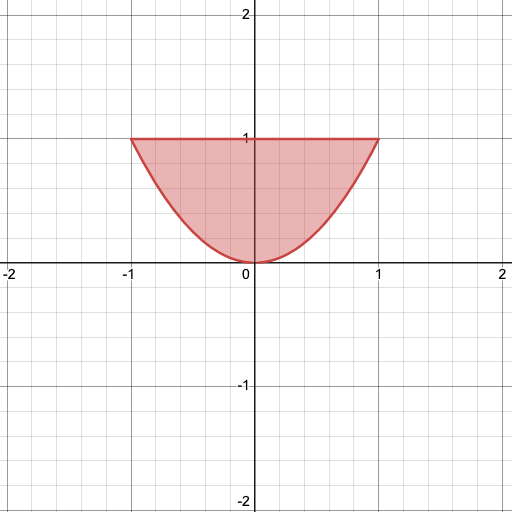
\includegraphics[width=0.8\linewidth]{figures/iii_img-2.png}
\end{center}

\columnbreak

\begin{center}
    \[
        \partial E
    .\]
    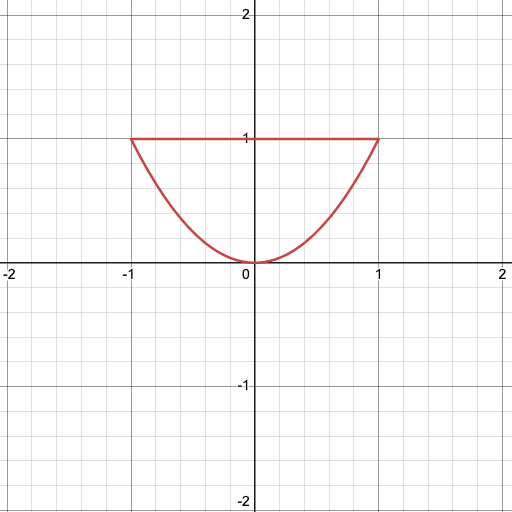
\includegraphics[width=0.8\linewidth]{figures/iii_img-3.png}
\end{center}
\end{multicols}

\section*{Problem 4}
\begin{proof}
    \begin{enumerate}[label=\roman*)]
        \item Suppose $V$ is open. Then for every point $\alpha \in V$, there is some $r_{\alpha} > 0$ such that $B_{r_{\alpha}}(\alpha) \subseteq V$. Since these balls are all open and $\alpha \in B_{r_{\alpha}}(\alpha)$,
        \[
            \bigcup_{\alpha \in V} B_{r_{\alpha}}(\alpha) = V
        .\]
        Suppose now there is collection of open balls whose union is $V$. Since the union of any collection of open sets is open, $V$ must be open.
        \item The same result does not hold. Specifically the reverse direction is not guranteed as the infinite union of closed sets can sometimes be open and not closed.
    \end{enumerate}
\end{proof}


\section*{Problem 5}
\begin{proof}
    Note that the inequality is trivial if $x \cdot y < 0$. Assume then that $x \cdot y \geq 0$. Then the left hand side is
    \begin{align*}
        (x \cdot y)^2 (|x| + |y|)^2 &= (x \cdot y)^2 (|x|^2 + 2|x||y| + |y|^2)
    \end{align*}
    and the right hand side is
    \begin{align*}
        |x|^2 |y|^2 |x + y|^2 = |x|^2 |y|^2 (|x|^2 + 2 x\cdot y + |y|^2).
    \end{align*}
    Since $x \cdot y > 0$, from Cauchy-Schwarz $x \cdot y \leq |x| |y|$. Thus the left hand side by applying Cauchy Schwarz multiple times gives
    \begin{align*}
        (x \cdot y)^2 (|x|^2 + 2|x||y| + |y|^2) &\leq |x|^2 |y|^2 |x|^2 + 2 (x \cdot y)(|x| |y|)(|x||y|) + |x|^2 |y|^2 |y|^2 \\
        &= |x|^2 |y|^2 (|x|^2 + 2 x \cdot y + |y|^2).
    \end{align*}
    Thus the LHS is smaller than the RHS.
\end{proof}

\section*{Problem 6}
\begin{enumerate}[label=\roman*)]
    \item Let $x \in \interior(A)$. Then there exists some nbhd $V$ of $x$ such that $V \subseteq A$. Since $A \subset B$, it follows $V \subset B$. Therefore $V$ is a nbhd of $x$ in $B$, meaning $x \in \interior(B)$.
    \item Let $x \in \interior(A \cap B)$. Then there exists some nbhd $V$ of $x$ such that $V \subseteq A \cap B$. But this means $V \subseteq A$ and $V \subseteq B$, therefore $V$ is a nbhd of $x$ in both $A$ and $B$. Therfore $x \in \interior(A)$ and $x \in \interior(B)$ meaning $x \in \interior(A) \cap \interior(B)$. Now let $x \in \interior(A) \cap \interior(B)$. Then there exists nbhds $V_A$ and $V_B$ of $x$ such that $V_A \subseteq A$ and $V_B \subseteq B$. Since the intersection of two open sets is open, $V_A \cap V_B$ is open and $V_A \cap V_B \subseteq A \cap B$. Therefore $V_A \cap v_B$ is a nbhd of $x$ in $A \cap B$ meaning $x \in \interior(A \cap B)$.

    \item Note that $\conj{A \cup B} = \interior((A \cup B)^c) = \interior(A^c \cap B^c)$. From $(ii)$ it follows $\conj{A \cup B} = \interior(A^c) \cap \interior(B^c) = \conj{A} \cup \conj{B}$.
\end{enumerate}

\end{document}
